\documentclass[12pt,a4paper]{article}
\usepackage{cmap}
\usepackage{amsmath}
\usepackage{mathtext}
\usepackage{titlesec}

\usepackage[utf8]{inputenc}
\usepackage[T2A]{fontenc}
\usepackage{wrapfig}
\usepackage[english, russian]{babel}
\usepackage[left=2cm,right=2cm,top=2cm,bottom=2cm]{geometry}
\usepackage{indentfirst}

\DeclareSymbolFont{T2Aletters}{T2A}{cmr}{m}{it}

%%% Работа с картинками
\usepackage{graphicx}  % Для вставки рисунков
\graphicspath{{imgs/}}  % папки с картинками

\usepackage{caption}
\captionsetup{labelsep=period, labelfont=bf}

\titleformat{\section}[block]
{\normalfont}{\thesection.}{0 cm}{}
\titleformat{\subsection}[block]
{\bfseries}{\thesubsection.}{0 cm}{}

\titlespacing{\section}{17pt}{14pt}{10pt}
\titlespacing{\subsection}{17pt}{14pt}{4pt}

\def \TITLE {Отчет о выполнении лабораторной работы №1.1.1}
\def \SUBTITLE {Измерение удельного сопротивления нихромовой проволоки}
\def \AUTHOR {Выполнил студент группы Б03-405\\ Тимохин Даниил}
\def \DATE {4 сентября 2024 г.}

\begin{document}

\begin{titlepage}
	\centering
	\vspace{5cm}
	{\scshape\large Московский физико-технический институт \\
	(НАЦИОНАЛЬНЫЙ ИССЛЕДОВАТЕЛЬСКИЙ УНИВЕРСИТЕТ)}
	
	\vspace{4cm}
	{\LARGE \TITLE}
	
	\vspace{1cm}
	{\Huge\bf \SUBTITLE }
	
	\vspace{1cm}
	\vfill
	
\begin{flushright}
	{\LARGE \AUTHOR}
\end{flushright}
	

	\vfill

	\DATE
\end{titlepage}

\newpage

\fontsize{12}{14}\selectfont

\section{ Аннотация}
В работе измеряется удельное сопротивление тонкой проволоки круглого сечения, изготовленной из нихромового сплава. Используются следующие методы измерений сопротивления: 1) определение углового коэффициента наклона зависимости напряжения на проволоке от тока
через неё, измеряемых с помощью аналоговых и цифровых вольтметров и амперметров, 2) измерение с помощью моста постоянного тока. Геометрические размеры образца измеряются с
помощью линейки, штангенциркуля и микрометра. Детально исследуется систематические и
случайные погрешности проводимых измерений. Отрабатываются навыки подтверждения теоретических зависимостей эксперементальными данными.

\section{ Теоритические сведенья}
Уделиное сопротивление определяется по формуле
\begin{equation}\label{Rho_eq}
\rho = R \frac{\pi d^2}{4l},
\end{equation}
где $R$ -- сопротивление проволки,  $d$ -- её диаметр, $l$ -- длина.

Согласно закону Ома напряжение $V$ и ток $I$ в образце связаны отношением
\begin{equation}\label{Om_eq}
V = RI.
\end{equation}

\begin{wrapfigure}{r}{0.4\textwidth}
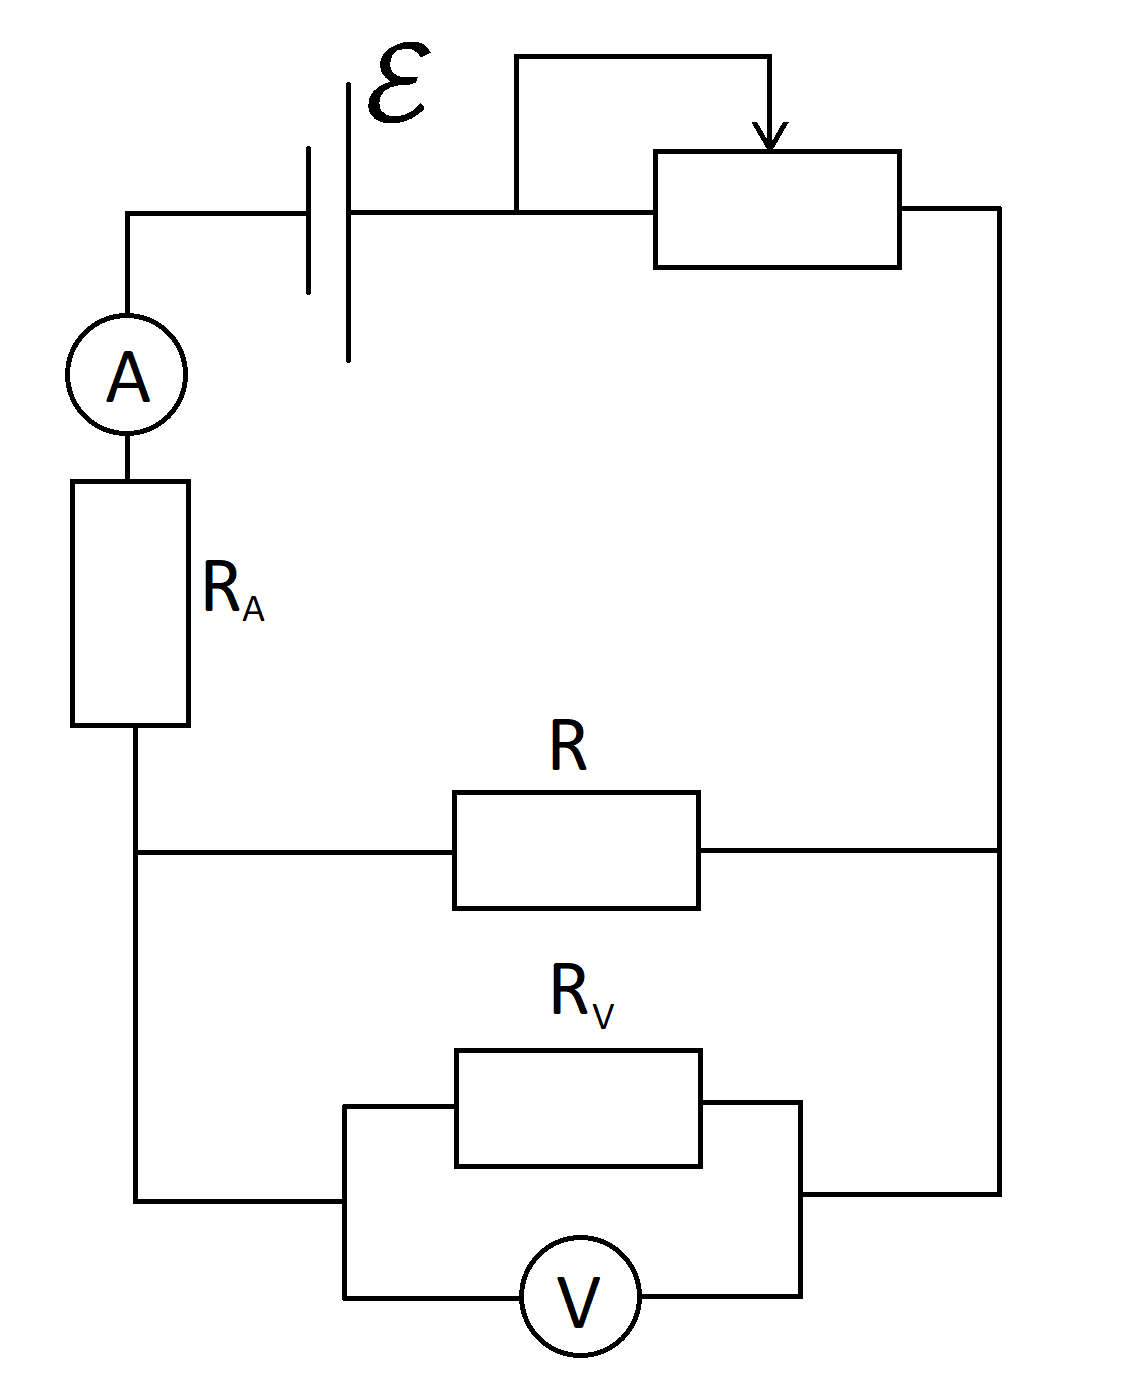
\includegraphics[width=0.34\textwidth]{imgs/scheme.png}
\caption{Схема измерения вольт-амперной характеристики проволки}
\label{fig:scheme}
\end{wrapfigure}
Для измеренмя напряжения и тока использовалась схема рис. \ref{fig:scheme}, так как обладала меньшей величиной поправки.

Ввиду неидеальности используемого вольтметра необходимо
учесть поправку на его конечное сопротивление $R_V$.  Показания амперметра $I_A$ и вольтметра $V_B$ связаны соотношением
\begin{equation}\label{Vb_eq}
V_B = R'I_A,
\end{equation}
где $R'$ — сопротивление параллельно соединенных проволоки и
вольтметра, причём $\frac 1 R' = \frac 1 R + \frac 1 R_V$, и $R_V \gg R,R'$. График зависимости $V_B(I_A)$ должен представлять прямую, угловой коэффициент которой есть $R'$, откуда сопротивление образца может быть найдено как
\begin{equation} \label{R_eq}
R = \frac {R_V R'} {R_V-R'} \approx R'\left(1+\frac{R'}{R_V}\right)
\end{equation}


Погрешность еденичного измерения параметра $\sigma _x$ $x$ будет расчитываться по формуле
\begin{equation}
    \sigma _x = \sqrt{ (\sigma _x ^{случ})^2 + (\Delta _x ^{сист})^2},
\end{equation}
где $\Delta _x ^{сист}$ -- систематическая погрешность, определяемая только параметрами прибора, а $\sigma _x ^{случ}$ -- случайная погрешность при измерениях. Введём $\overline{x}=\frac{1}{N}\sum x_i$, где N -- количество измерений.  Согласно теории вероятностей случайную погрешность одного измерения при малых N можно определить по формуле
\begin{equation}
\sigma _x ^{случ} = \sqrt{\frac{1}{N-1} \sum \left( x_i - \overline{x} \right)^2}
\end{equation}
из неё можно получить значение случайной погрешности среднего $\sigma _{\overline{x} ^{случ}} = \frac{\sigma _x ^{случ}}{\sqrt{N}}$

\section{ Оборудование и инструментальные погрешности}
{\bfseries Линейка:} $\Delta _{лин} = \pm 1$ мм (по цене деления). При определении положений контактов имеется дополнительная погрешность, которая может быть оценена как $\Delta _{лин} = \pm 2$ мм

{\bfseries Штангенциркуль:} $\Delta _{шт} = \pm$0,1 мм (маркировка производителя).

{\bfseries Микрометр:} $\Delta _{шт} = \pm$0,01 мм (маркировка производителя).
%\newpage
{\bfseries Вольтметр:} 
\begin{table}[h!]
\quad\quad
\begin{tabular}{|p{6cm}|c|}
\hline
Система & Магнито-электрическая \\ \hline
Класс точности & 0,2  \\ \hline
Шкала & линейная,
150 делений  \\ \hline
Предел измерерний & 0,6 В  \\ \hline
Цена деления & $4 \cdot 10^{-3}$ B = 4 мВ \\ \hline
Чувствительность & 250 дел./В \\ \hline
Внутреннее споротивление & $R_V$ = 10 кОм  \\ \hline
Погрешность при считывании \newline со шкалы(0,5 цены деления) & $\pm 4$ мВ \\ \hline
Макс. погрешность\newline (согласно классу точности) 
 & $\pm 1,2$ мВ (0,2 \%) \\ \hline
\end{tabular}
\end{table}

{\bfseries Амперметр:} 
\begin{table}[h]
\quad\quad
\begin{tabular}{|p{6cm}|p{6cm}|}
\hline
Система & Цифровая \\ \hline
Предел измерерний &  500 мА  \\ \hline
Разрядность дисплея & 5 ед. \\ \hline
Внутреннее сопротивление & $R_A$ = 1,2 Ом \\ \hline
Погрешнось (при комнатной
температуре, согласно паспорту
прибора) 
 & $\Delta _{A} = \pm (0,002 \cdot X + 2k)$ \newline где $X$ — измеряемая величина, $k$ — единица младшего разряда ($k$ = 0,01 мА). \\ \hline
\end{tabular}
\end{table}

При измерениях в диапазоне от 10 мА до 200 мА погрешность амперметра составила соответственно от $\Delta _{A} = \pm$0,04 мА (0.4\%) до $\Delta _{A} = \pm$0,4 мА (0.2\%).


В диапазоне измерения $R$ от 1 до 10 Ом относительная поправка $\frac{R'}{R_V}$ к сопротивлению согласно ф-ле (\ref{R_eq}) составляет от 0,01\% (при $R$ = 1 ом и $R_V$ = 10 кОм) до 0,1\% (при $R$ = 10 Ом и $R_V$ = 10 кОм). Следовательно, данная поправка заведомо меньше погрешности измерений (0,5\% для вольтметра), поэтому примем далее, что неидеальность вольтметра не оказывает влияния на измерение сопротивления:
\begin{equation}\label{Rarx_eq}
R \approx R'.
\end{equation}

{\bfseries Мост постоянного тока Р4833:}

\quad Класс точности: 0,1

\quad Разрядность магазина сопротивлений: 5 ед.

\quad Используемый диапазон измерений: $10^{-4}$ – 10 Ом (для множителя $N$ = $10^{-2}$).

\quad Погрешность измерений в используемом диапазоне: $\pm$0,010 Ом.

\section{ Результаты измерений и обработка данных}
\subsection{Измерение диаметра $d$ проволоки.}
Измерения проводились штангенциркулем и микрометром многократно на разных участках
проволоки. При измерении штангенциркулем получено $d$ = 0,4 мм для каждого из $N$ = 10
измерений. При измерении микрометром выявлен разброс в показаниях, см. табл. 1
\begin{table}[!ht]
    \label{tbl:d}
     \caption{\newline Измерения диаметра проволоки микрометром.
    }
    \centering
    \begin{tabular}{|l|l|l|l|l|l|l|l|l|l|l|}
    \hline
        $N$, изм & 1 & 2 & 3 & 4 & 5 & 6 & 7 & 8 & 9 & 10 \\ \hline
        $d$, мм & 0.37 & 0.39 & 0.37 & 0.36 & 0.36 & 0.36 & 0.37 & 0.37 & 0.36 & 0.38 \\ \hline
    \end{tabular}
\end{table}

Среднее значение диаметра $\overline{d}=\frac{\sum d_i}{N}=$0,369 мм.

Стандартное отклонение: $\sigma{_d} = \sqrt{\frac{1}{N-1}\sum (d_i-\overline{d})^{2}}$=0,0099 мм

Случайная погрешность среднего: $\sigma _{\overline{d}} = \frac{\sigma _d}{\sqrt{N}}$= 0.0031 мм

С учётом инструментальной погрешности $\Delta _{мкм} = \pm$0,01 мм погрешность измерения диаметра может быть вычислена как $\sigma ^{полн} _{\overline{d}} = \sqrt{ \sigma ^{2} _{\overline{d}} + \Delta ^2 _{мкм}} = $ 0.0105 мм

\textit{Окончательные результаты измерения диаметра проволоки:}
\begin{center}
{ Штангенциркулем: $d$ = 0,4 $\pm$ 0,1 мм}

{ Микрометром: \underline{$d$ = 0,37 $\pm$ 0,01 мм} ($\varepsilon _d$ = 3,7\%)}
\end{center}
\subsection{ Измерение сопротивления проволоки.}

Результаты измерений зависимостей показаний вольтметра $V_B$ от показаний амперметра $I_A$ в схеме рис. \ref{fig:scheme} при разных длинах $l$ образца представлены в табл. 2. Соответствующие графики зависимостей изображены на рис. 2.

По графику убеждаемся, что экспериментальные данные с хорошей точностью (в пределах
инструментальных погрешностей опыта) ложатся на теоретическую прямую $V=RI$, исходящую из начала координат.

Пользуясь методом наименьших квадратов, строим аппроксимирующие прямые $V_B=\overline{R}I_A$,
определяя их угловой коэффициент по формуле
\begin{equation}
    \overline{R}=\frac{\langle IV \rangle}{\langle I^2 \rangle}.
\end{equation}

\begin{table}[!ht]
    \label{tbl:tb2}
     \caption{\newline Зависимость $V_B$ от $I_A$ для разных длин проволоки $l$.}
    \centering
    \begin{tabular}{|p{1.3cm}|l|l|p{1.3cm}|l|l|p{1.3cm}|l|l|}
    \hline 
        \multicolumn{3}{|c|}{ $l$ = 50 $\pm$ 0,2 см} & \multicolumn{3}{|c|}{ $l$ = 30 $\pm$ 0,2 см} & \multicolumn{3}{|c|}{ $l$ = 20 $\pm$ 0,2 см} \\ \hline
        {V, дел \newline 4 $\frac {мВ} {дел}$} & V, мВ & I, мА & {V, дел \newline 4 $\frac {мВ} {дел}$} & V, мВ & I, мА & {V, дел \newline 4 $\frac {мВ} {дел}$} & V, мВ & I, мА \\ \hline
        141 & 564 & 112.94 & 84 & 336 & 111.57 & 56.5 & 226 & 111.7 \\ \hline
        132 & 528 & 105.79 & 75 & 300 & 100.7 & 51 & 204 & 100.34 \\ \hline
        113 & 452 & 90.58 & 68 & 272 & 90.31 & 46 & 184 & 90.03 \\ \hline
        100 & 400 & 80.1 & 61 & 244 & 81.6 & 41 & 164 & 80.06 \\ \hline
        88 & 352 & 70.83 & 53 & 212 & 70.7 & 36 & 144 & 70.77 \\ \hline
        75 & 300 & 60.17 & 45 & 180 & 60.13 & 31 & 124 & 60.7 \\ \hline
        81.5 & 326 & 65.23 & 49 & 196 & 64.82 & 33 & 132 & 65.2 \\ \hline
        94 & 376 & 75.36 & 51 & 204 & 75.01 & 38 & 152 & 75.22 \\ \hline
        106 & 424 & 85.24 & 64 & 256 & 85.33 & 43 & 172 & 85.39 \\ \hline
        118.5 & 474 & 95.09 & 72 & 288 & 95.9 & 48.5 & 194 & 95.97 \\ \hline
        133 & 532 & 106.61 & 79.5 & 318 & 106.01 & 53 & 212 & 105.6 \\ \hline
        148 & 592 & 118.66 & 86 & 344 & 115.3 & 58 & 232 & 115.05 \\ \hline
    \end{tabular}
\end{table}

Случайную погрешность определения углового коэффициента вычисляем как
\begin{equation}
    \sigma ^{сл} _{R} = \sqrt{ \frac{1}{n-1} \left(\frac{\langle V^2 \rangle}{\langle I^2 \rangle} - \overline{R}^2\right) }
\end{equation}
(здесь $n$ = 10 – число точек на графике).

Оценим возможную систематическую погрешность, обусловленную инструментальными
погрешностями приборов. Предполагая, что при всех измерениях относительная погрешность
приборов одинакова, оценим погрешность вычисления частного $R=V/I$ при максимальных
значениях $V$ и $I$:
\begin{equation}
    \Delta ^{сист} _{R} \sim R \sqrt{ \left( \frac {\Delta V}{V_{max}} \right)^2 + \left( \frac {\Delta I}{I_{max}} \right)^2 }.
\end{equation}
Полная погрешность измерения $R$ не превосходит значения
\begin{equation}
    \sigma ^{полн} _{R} \leq \sqrt{ ( \sigma ^{сл} _R )^2 + ( \Delta ^{сист} _{R} )^2 }.
\end{equation}

Результаты сведены в табл. 3. Там же для сравнения приведены результаты измерения $R$ с
помощью моста постоянного тока Р4833 с учётом его погрешности.

\begin{table}[!ht]
    \label{tb:tb3}
    \caption{\newline Результаты измерения сопротивления проволоки двумя методами}
    \centering
    \begin{tabular}{|l|l|l|l|l|l|}
    \hline
        l, см & $\overline{R}$, Ом & $\sigma ^{полн} _{R}$, Ом & $\Delta ^{сист} _{R}$, Ом & $\sigma ^{полн} _{R}$, Ом & $R_{мост}$, Ом \\ \hline
        50 & 4,988 & 0,014  & 0,011  & 0,018 & 5,009$\pm$0,010 \\ \hline
        30 & 3,019  & 0,021 & 0,007 & 0,022 & 3,009$\pm$0,010 \\ \hline
        20 & 2,025 & 0,012  & 0,006  & 0,013 & 2,03$\pm$0,010 \\ \hline
    \end{tabular}
\end{table}

Видно, что случайная составляющая измерения сопротивления мала, а основной вклад вносят систематические приборные погрешности. Контрольные измерения с помощью моста дают
заниженные результаты, но все отклонения находятся в пределах $\pm2 \sigma ^{полн} _{R}$.
\begin{figure}[htbp]
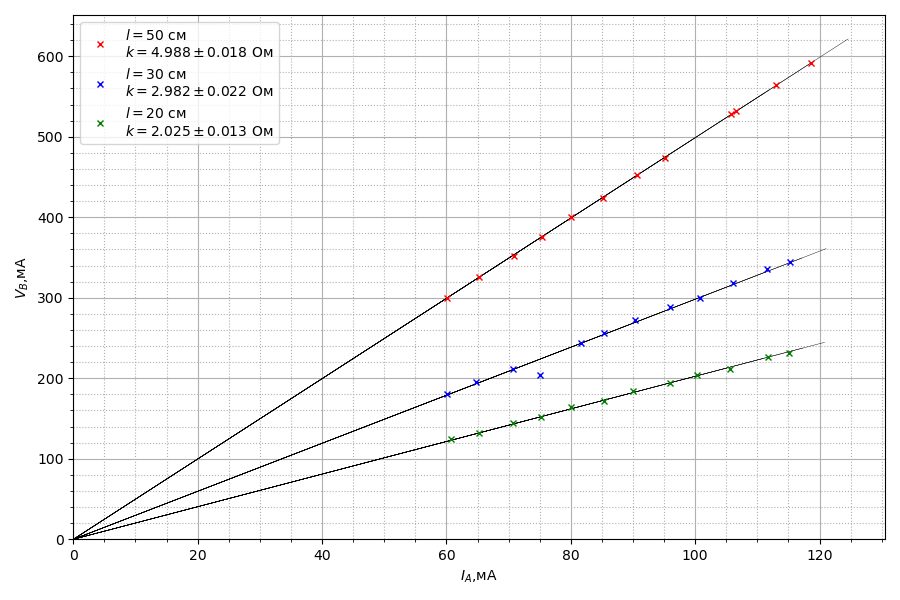
\includegraphics[width=0.95\textwidth]{imgs/graphic.png}
\caption{Результаты измерений напряжения $V_B$ в зависимости от тока $I_A$ для проволок разной длины $l$ и
их линейная аппроксимация $y=kx$. Кресты погрешности не изображены, так как $V_B\gg\sigma_{V_B}$ и сами кресты будут намного меньше длений графика.}
\label{fig:graphic}
\end{figure}

\subsection{ Вычисление удельного сопротивления}
По формуле (\ref{Rho_eq}) находим удельное сопротивление материала проволоки, используя значения
$\overline{R}$, полученные п. 4.2. Для оценки погрешности воспользуемся формулой
\begin{equation}
    \sigma _{\rho} = \rho\sqrt{ \left( \frac{\sigma _R}{R} \right)^2 + \left( 2\frac{\sigma _d}{d} \right)^2 +\left( \frac{\sigma _l}{l} \right)^2 }
\end{equation}
Проведя вычисления получим:
\begin{table}[!ht]
    \quad\quad\begin{tabular}{|l|l|}
    \hline
    $N$ опыта & $\rho$, $10^{-6}$ Ом $\cdot$ м \\ \hline
    1 & 1.067$\pm$0.06\\ \hline
    2 & 1.063$\pm$0.06\\ \hline
    3 & 1.083$\pm$0.06\\ 
    \hline
    \end{tabular}
\end{table}

Усредняя результаты 3-х опытов, окончательно получим:

{\centering \underline{$\overline{\rho}$ = $(1,08 \pm 0,06)\cdot 10^{-6}$ Ом $\cdot$ м} ($\varepsilon_{\rho}$ = 6\%)}

Из $\varepsilon_{\rho}$ видно, что наибольший вклад сделала $\varepsilon_{d}$, так как она учитываетя дважды в формуле (10) по законам теории вероятностей.
\newpage

\section{ Обсуждение результатов и выводы}
В работе получено значение удельного сопротивления образца проволоки из нихромового
сплава с точностью ~6\%. Табличные значения для нихрома лежат в диапазоне
$\rho_{табл} = 0,97~\ldots~1,14 \cdot 10^{-6}$ Ом $\cdot$ м  в зависимости от состава. Измеренные значения
$\rho = (1,08 \pm 0,06) \cdot 10^{-6}$ Ом $\cdot$ м попадают в этот диапазон в пределах одного стандартного отклонения, однако погрешность результата не позволяет определить марку сплава.

Использованный в работе метод измерения сопротивлений позволил получить значения $R$
образцов с довольно высокой точностью (0,5\%), которая ограничивалась в основном погрешностью аналогового вольтметра. Величина случайной погрешности $\sigma ^{ck} _{R}$
сл, найденная в п. 4.2., показывает, что использование более совершенных измерительных приборов позволило бы довести точность измерения по данной методике до 0,1–0,2\% (при неизменном количестве измерений), что сопоставимо с точностью измерений с помощью мостовой схемы.

Точность измерения удельного сопротивления $\rho$ существенно ограничивается измерением
диаметра проволоки. Поскольку случайная ошибка измерения диаметра оказалась меньше
цены деления прибора (микрометра), уточнение значения диаметра за счет многократных измерений невозможно. По той же причине не удалось проверить, насколько однородной является проволока по сечению.
\end{document}